\documentclass[10pt]{standalone}
\usepackage[utf8]{inputenc}
\usepackage{pgf,tikz}
\usepackage{mathrsfs}
\usetikzlibrary{arrows,positioning,calc}
\pagestyle{empty}
\usepackage[T1]{fontenc} % font encoding
\usepackage[utf8]{inputenc} % input encoding
%\usepackage{noto}
\usepackage[largesc]{newtxtext} %
\usepackage[varqu,varl]{zi4}% inconsolata
\usepackage{cabin}% sans serif
\usepackage[vvarbb]{newtxmath}
\useosf % use oldstyle figures except in math

%\tikzset{every picture/.style={scale=0.3,every picture/.style={}}}
\tikzset{main base/.style={draw,thick,text centered, }, }
\tikzset{main node/.style={rectangle, draw,rounded corners,main base}, }
%      
%\tikzset{main verb/.style={minimum size=1cm}, }
%\tikzset{linea/.style={-triangle 90}, }
%\tikzset{main node2/.style={rectangle, draw,thick,
%    text width=7em, text centered, rounded corners, minimum height=3em}, }
\tikzset{main node2/.style={main node,
    text width=7em, minimum height=3em}, }
\tikzset{main verb/.style={minimum size=1cm}, }
\tikzset{linea/.style={-triangle 90,thick,draw}}
%\tikzset{linea/.style={-triangle 90,thick,draw}}
\tikzset{linea2/.style={-triangle 90,draw}}
\tikzset{primo/.style={circle,draw,inner sep=0pt,minimum size=1pt,thick}, }
\tikzset{
    start-end/.style={
        draw,
        rectangle,
        rounded corners,main base,
    } ,
    input/.style={ % requires library shapes.geometric
        draw,
        trapezium,
        trapezium left angle=60,
        trapezium right angle=120,main base
    },
    operation/.style={
        draw,thick,
        rectangle,main base,
    },
    loop/.style={ % requires library shapes.misc
        draw,
        chamfered rectangle,
        chamfered rectangle xsep=2cm
    },
    decision/.style={ % requires library shapes.geometric
        draw,
        diamond,
        aspect=#1,main base
    },
    decision/.default=1,
    print/.style={ % requires library shapes.symbols
        draw,
        tape,
        tape bend top=none
    },
    connection/.style={
        draw,
        circle,
        radius=5pt,
    },
    process rectangle outer width/.initial=0.15cm,
    predefined process/.style={
        rectangle,
        draw,
        append after command={
        \pgfextra{
          \draw
          ($(\tikzlastnode.north west)-(0,0.5\pgflinewidth)$)--
          ($(\tikzlastnode.north west)-(\pgfkeysvalueof{/tikz/process rectangle outer width},0.5\pgflinewidth)$)--
          ($(\tikzlastnode.south west)+(-\pgfkeysvalueof{/tikz/process rectangle outer width},+0.5\pgflinewidth)$)--
          ($(\tikzlastnode.south west)+(0,0.5\pgflinewidth)$);
          \draw
          ($(\tikzlastnode.north east)-(0,0.5\pgflinewidth)$)--
          ($(\tikzlastnode.north east)+(\pgfkeysvalueof{/tikz/process rectangle outer width},-0.5\pgflinewidth)$)--
          ($(\tikzlastnode.south east)+(\pgfkeysvalueof{/tikz/process rectangle outer width},0.5\pgflinewidth)$)--
          ($(\tikzlastnode.south east)+(0,0.5\pgflinewidth)$);
        }  
        },
        text width=#1,
        align=center
    },
    predefined process/.default=1.75cm,
    man op/.style={ % requires library shapes.geometric
        draw,
        trapezium,
        shape border rotate=180,
        text width=2cm,
        align=center,
    },
    extract/.style={
        draw,
        isosceles triangle,
        isosceles triangle apex angle=60,
        shape border rotate=90
    },
    merge/.style={
        draw,
        isosceles triangle,
        isosceles triangle apex angle=60,
        shape border rotate=-90
    },
}

\begin{document}
  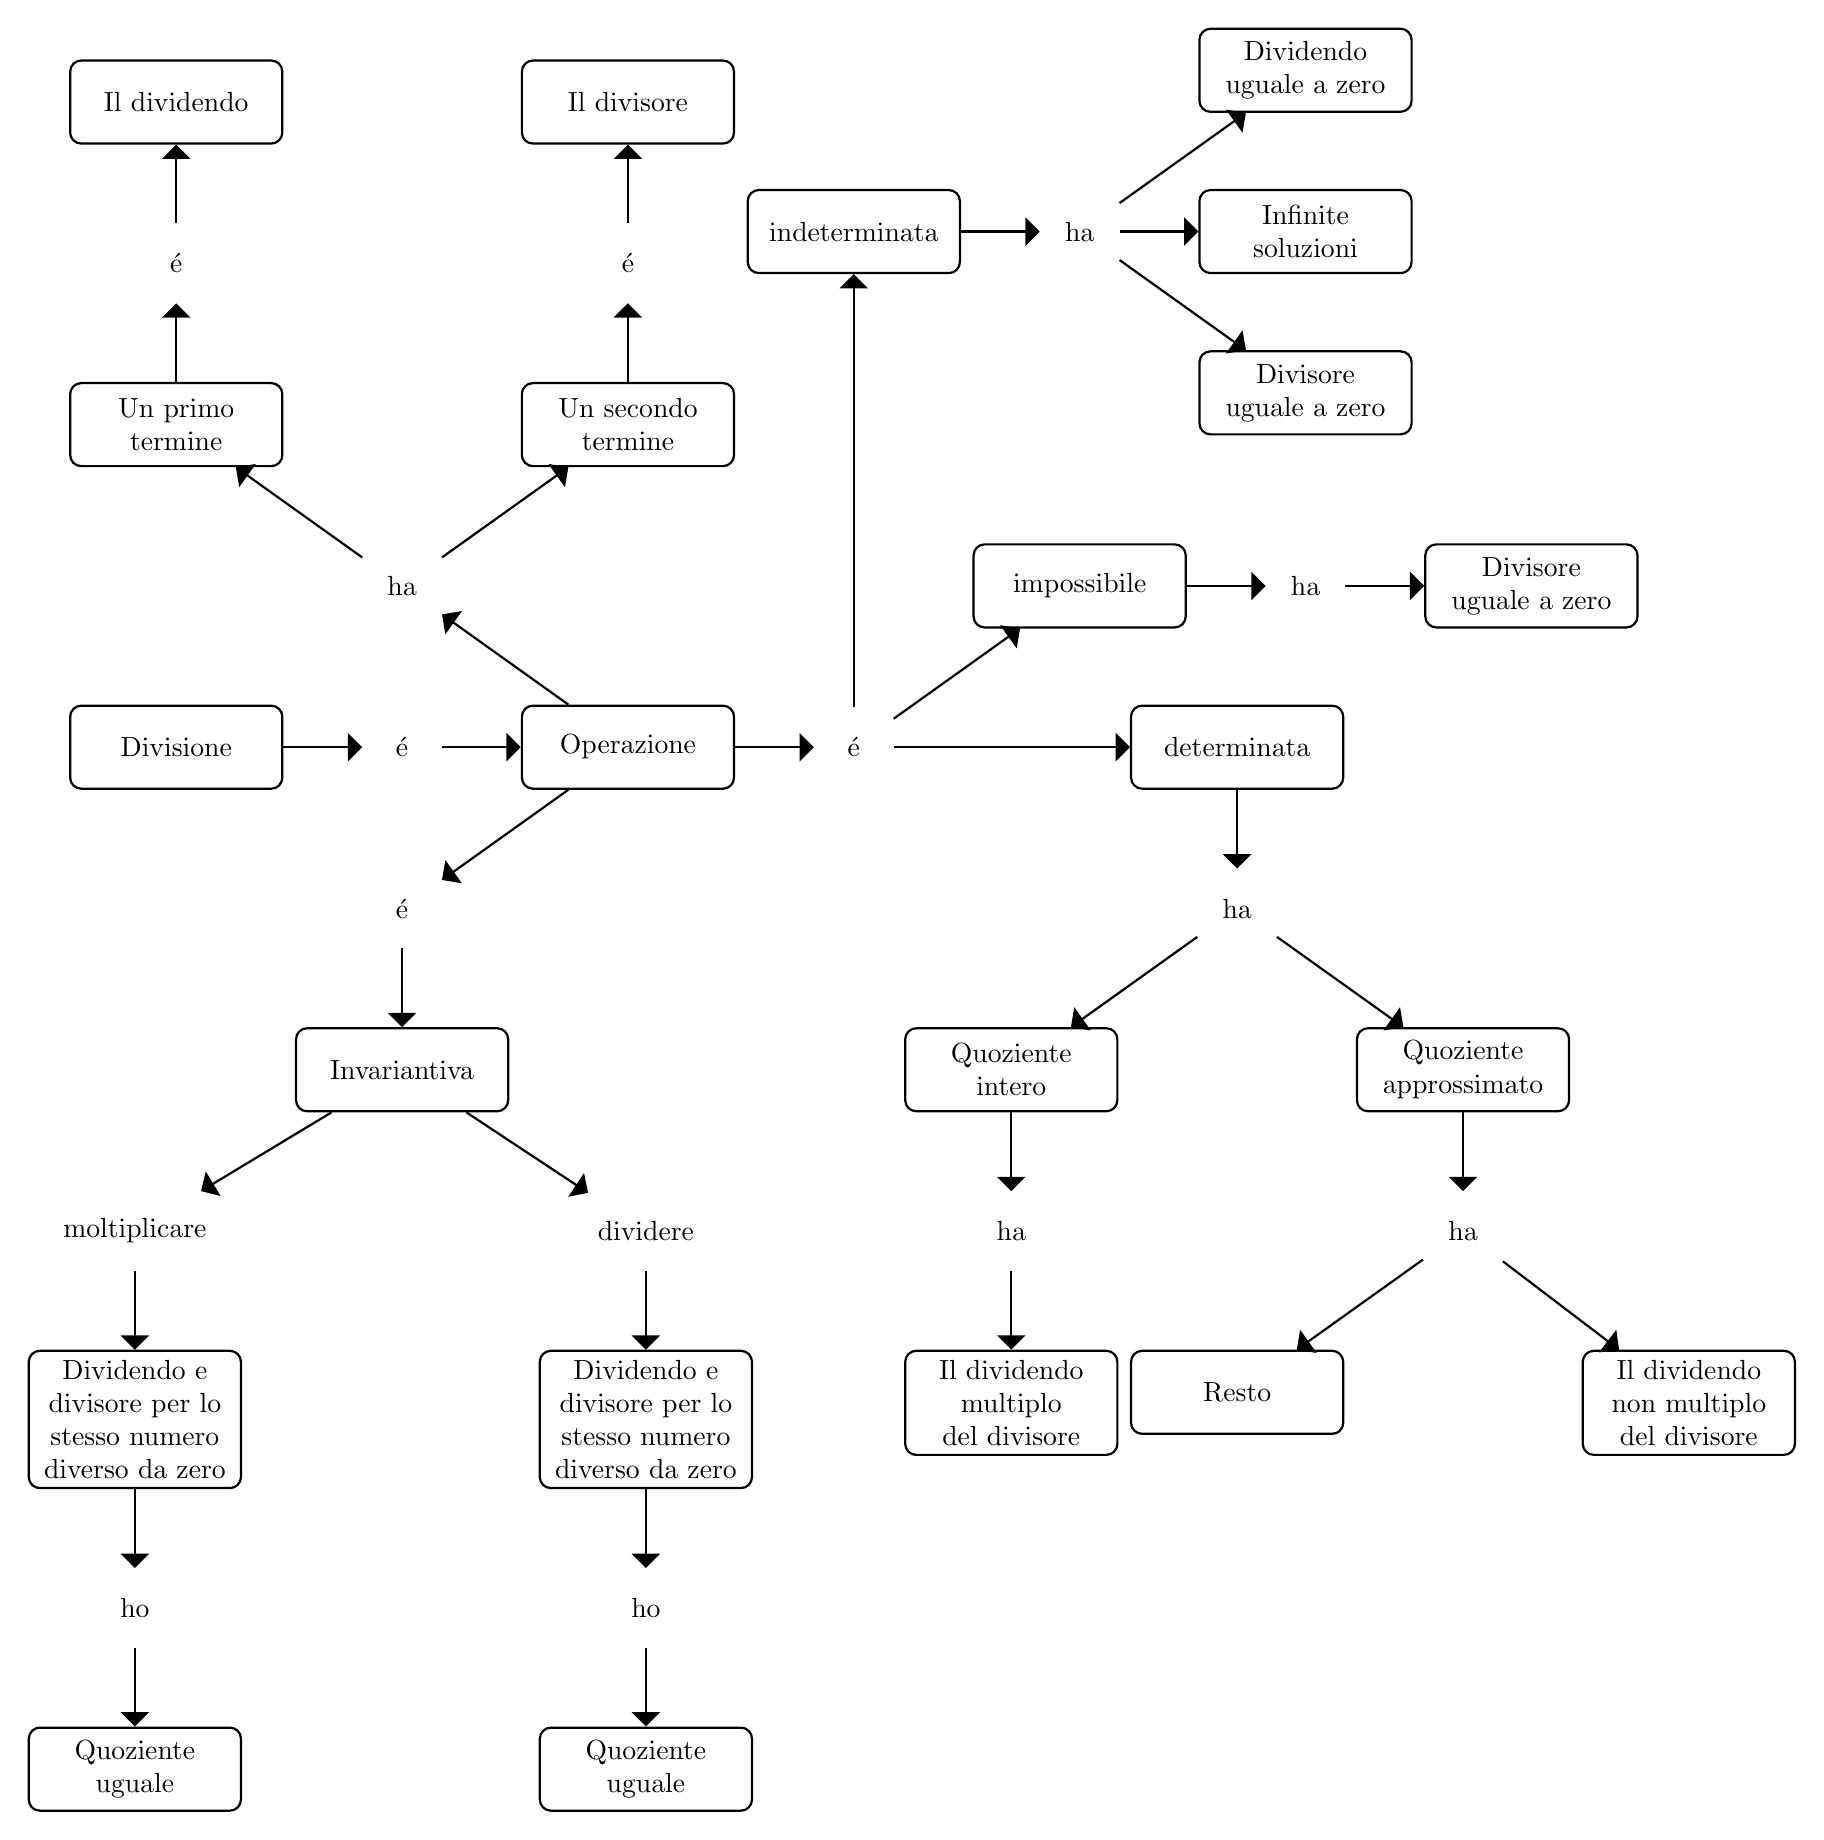
\begin{tikzpicture}
 \tikzset{every picture/.style={scale=0.3,every picture/.style={}}}
 \tikzset{main base/.style={draw,thick,text centered, }, }
 \tikzset{main node/.style={rectangle, draw,rounded corners,main base}, }
 %      
 %\tikzset{main verb/.style={minimum size=1cm}, }
 %\tikzset{linea/.style={-triangle 90}, }
 %\tikzset{main node2/.style={rectangle, draw,thick,
 %    text width=7em, text centered, rounded corners, minimum height=3em}, }
 \tikzset{main node2/.style={main node,
 		text width=7em, minimum height=3em}, }
 \tikzset{main verb/.style={minimum size=1cm}, }
 \tikzset{linea/.style={-triangle 90,thick,draw}}
 %\tikzset{linea/.style={-triangle 90,thick,draw}}
 \tikzset{linea2/.style={-triangle 90,draw}}
 \tikzset{primo/.style={circle,draw,inner sep=0pt,minimum size=1pt,thick}, }
 \tikzset{
 	start-end/.style={
 		draw,
 		rectangle,
 		rounded corners,main base,
 	} ,
 	input/.style={ % requires library shapes.geometric
 		draw,
 		trapezium,
 		trapezium left angle=60,
 		trapezium right angle=120,main base
 	},
 	operation/.style={
 		draw,thick,
 		rectangle,main base,
 	},
 	loop/.style={ % requires library shapes.misc
 		draw,
 		chamfered rectangle,
 		chamfered rectangle xsep=2cm
 	},
 	decision/.style={ % requires library shapes.geometric
 		draw,
 		diamond,
 		aspect=#1,main base
 	},
 	decision/.default=1,
 	print/.style={ % requires library shapes.symbols
 		draw,
 		tape,
 		tape bend top=none
 	},
 	connection/.style={
 		draw,
 		circle,
 		radius=5pt,
 	},
 	process rectangle outer width/.initial=0.15cm,
 	predefined process/.style={
 		rectangle,
 		draw,
 		append after command={
 			\pgfextra{
 				\draw
 				($(\tikzlastnode.north west)-(0,0.5\pgflinewidth)$)--
 				($(\tikzlastnode.north west)-(\pgfkeysvalueof{/tikz/process rectangle outer width},0.5\pgflinewidth)$)--
 				($(\tikzlastnode.south west)+(-\pgfkeysvalueof{/tikz/process rectangle outer width},+0.5\pgflinewidth)$)--
 				($(\tikzlastnode.south west)+(0,0.5\pgflinewidth)$);
 				\draw
 				($(\tikzlastnode.north east)-(0,0.5\pgflinewidth)$)--
 				($(\tikzlastnode.north east)+(\pgfkeysvalueof{/tikz/process rectangle outer width},-0.5\pgflinewidth)$)--
 				($(\tikzlastnode.south east)+(\pgfkeysvalueof{/tikz/process rectangle outer width},0.5\pgflinewidth)$)--
 				($(\tikzlastnode.south east)+(0,0.5\pgflinewidth)$);
 			}  
 		},
 		text width=#1,
 		align=center
 	},
 	predefined process/.default=1.75cm,
 	man op/.style={ % requires library shapes.geometric
 		draw,
 		trapezium,
 		shape border rotate=180,
 		text width=2cm,
 		align=center,
 	},
 	extract/.style={
 		draw,
 		isosceles triangle,
 		isosceles triangle apex angle=60,
 		shape border rotate=90
 	},
 	merge/.style={
 		draw,
 		isosceles triangle,
 		isosceles triangle apex angle=60,
 		shape border rotate=-90
 	},
 }
    \node[main node2] (1) {Divisione};
    \node[main verb] (2) [right=of 1]  {\'{e}};
    \node[main node2] (3) [right=of 2] {Operazione};
    \node[main verb] (4) [above left=of 3]  {ha};
    \node[main verb] (5) [right=of 3]  {\'{e}};    
    \node[main verb] (6) [below left=of 3]  {\'{e}};
        
\node[main node2] (7) [above left=of 4]  {Un primo termine};
    
\node[main node2] (8) [above right=of 4]  {Un secondo termine};

\node[main node2] (9) [above =5.5cm and 0cm of 5]  {indeterminata};
\node[main node2] (10) [right=2cm and 3cm of 5]  {determinata};    
\node[main node2] (11) [above right=of 5]  {impossibile};
\node[main node2] (12) [below=of 6]  {Invariantiva}; 
\node[main verb] (13) [above=of 7]  {\'{e}}; 
\node[main verb] (14) [above=of 8]  {\'{e}};     
%\node[main verb] (15) [above right=of 9]  {ha};
    
\node[main verb] (16) [right=of 9]  {ha};
\node[main verb] (17) [below=of 10]  {ha}; 
\node[main verb] (18) [right=of 11]  {ha}; 
\node[main verb] (19) [below left=of 12]  {moltiplicare};
    
\node[main verb] (20) [below right=of 12]  {dividere};
\node[main node2] (21) [above=of 13]  {Il dividendo};   
\node[main node2] (22) [above=of 14]  {Il divisore};
\node[main node2] (23) [right=of 16]  {Infinite soluzioni};
\node[main node2] (24) [above right=of 16]  {Dividendo uguale a zero};
    
\node[main node2] (25) [below right=of 16]  {Divisore uguale a zero};
\node[main node2] (26) [below left=of 17]  {Quoziente intero};
    
\node[main node2] (27) [below right=of 17]  {Quoziente approssimato};
\node[main node2] (28) [right=of 18]  {Divisore uguale a zero};   
\node[main node2] (29) [below=of 19]  {Dividendo e divisore per lo stesso numero diverso da zero};   
\node[main node2] (30) [below=of 20]  {Dividendo e divisore per lo stesso numero diverso da zero};   
\node[main verb] (31) [below=of 26]  {ha};
\node[main verb] (32) [below=of 27]  {ha};
\node[main verb] (33) [below=of 29]  {ho};
\node[main verb] (34) [below=of 30]  {ho};
\node[main node2] (35) [below=of 31]  {Il dividendo multiplo del divisore}; 
\node[main node2] (36) [below  left=of 32]  {Resto};
    
\node[main node2] (37) [below right=of 32]  {Il dividendo non multiplo del divisore};
\node[main node2] (38) [below=of 33]  {Quoziente uguale};
\node[main node2] (39) [below=of 34]  {Quoziente uguale};
%\node[main verb] (4) [above right=1.5cm and 1cm  of 3]  {ha};

\foreach \x /\y in{1/2,2/3,3/4,3/5,3/6,4/7,4/8,5/9,5/10,5/11,6/12,7/13,8/14,9/16,10/17,11/18,12/19,12/20,13/21,14/22,16/23,16/24,16/25,17/26,17/27,18/28,19/29,20/30,26/31,27/32,29/33,30/34,31/35,32/36,32/37,33/38,34/39}
  \path[linea] (\x) edge node {} (\y);
%  
\end{tikzpicture}
\end{document}